%%%%%%%%%%%%%%%%%%%%%%%%%%%%%%%%%%%%%%%%%%%%%%%%%%%%%%%%%%%%%%%%%%%%%%%%%%%
%%%                         INTRODUÇÃO                                  %%%
%%%%%%%%%%%%%%%%%%%%%%%%%%%%%%%%%%%%%%%%%%%%%%%%%%%%%%%%%%%%%%%%%%%%%%%%%%%

\chapter{Introdução}

\setlength{\parskip}{0.3cm}
%\thispagestyle{headings}

% Contextualização, relevância (importância, justificativa, necessidade) do problema
Os problemas impostos pela pandemia do COVID-19 incluíram a falta de conhecimento suficiente para a compreensão da importância das ameaças biológicas e para a preparação médica, apesar dos avanços científicos e tecnológicos já alcançados na área em questão. Em vista disso, o conhecimento prévio sobre os agentes biológicos com potencial para causar pandemias, tem o poder de melhorar substancialmente uma preparação pré-pandemia~\cite{behl_threat_2022}.

Diante disso, a bioinformática, que é a junção de métodos computacionais e técnicas estatísticas com o objetivo de extrair informações de dados biológicos brutos, desempenha um papel fundamental na interpretação de dados genômicos e na compreensão de processos evolutivos. % Completar aqui: , podendo assim facilitar na tomada de decisão daqueles que são responsáveis...
Segundo~\citeauthor{barry_phylogenetic_analysis_2006} os métodos filogenéticos podem ser usados para analisar os dados da sequência de nucleotídeos de forma que a ordem de descendência de cepas relacionadas possa ser determinada. Quando associada à análise filogenética apropriada, a epidemiologia molecular tem o potencial de elucidar os mecanismos que levam a surtos microbianos e epidemias.''

A reconstrução filogenética é uma das abordagens amplamente utilizadas na análise da evolução de espécies, que permite investigar as relações evolutivas entre diferentes linhagens de vírus. Essas observações são realizadas com base em dados como sequências de \gls{dna} e \gls{rna}. Essas sequências são formadas por blocos fundamentais chamados de nucleotídeos, que são compostos por uma base nitrogenada, um açúcar e um grupo fosfato. As bases presentes nos nucleotídeos do \gls{dna} são adenina (A), timina (T), citosina (C) e guanina (G), enquanto no \gls{rna} a base timina é substituída pela uracila (U)~\cite{alberts_molecular_2002}.

Uma das principais formas de análise filogenética é realizada através da árvore filogenética, onde são representadas as relações evolutivas entre um conjunto de espécies. De acordo com~\citeauthor{morrison_tree_thinking} elas tem função importante porque apresentam de forma sucinta e particular a evolução dos descendentes partindo de ancestrais em comum.

A semelhança genética entre vários vírus infecciosos e mortais fornece uma visão do fato de que o \gls{rna} é a chave para discernir e marcar os possíveis patógenos que podem causar uma pandemia. Embora um padrão geral e motivos conservados possam ser observados em ancestrais imediatos, as regiões não conservadas das sequências são o resultado da acumulação de mutações, seja por inserção ou deleção de um ou vários nucleotídeos ou por substituição pontual de um nucleotídeo por outro. A fonte principal de mutações em vírus são percalços na replicação e a recombinação de \gls{rna}~\cite{behl_threat_2022}.

Apesar da utilidade da filogenética e dos softwares comerciais e públicos disponíveis para análises filogenéticas, os métodos filogenéticos são muitas vezes aplicados de forma inadequada. Mesmo quando aplicados adequadamente, são mal explicados e, portanto, mal compreendidos.~\cite[p. 1]{barry_phylogenetic_analysis_2006} Além disso, por trabalhar com grandes quantidades de dados, os métodos utilizados devem ser avaliados também em relação ao seu custo computacional.

Na busca de trabalhos relacionados, vários métodos foram encontrados, e a seguir são apresentados.

O método de \gls{ml} (ou \textit{Maximum Likelihood}), não é exclusivo da filogenia, mas sim uma abordagem estatística. A sua aplicação em filogenia consiste em avaliar a probabilidade de que o modelo de evolução escolhido gere os dados observados, que são por exemplo, características de um organismo. Essa proposta foi utilizada nos seguintes trabalhos:
\begin{itemize}
  \item \citeauthor{behl_threat_2022}
  \item \citeauthor{fall_genetic_diversity_2021}
  \item \citeauthor{shabbir_comprehensive_2020}
  \item \citeauthor{hudu_hepatitis_2018}
  \item \citeauthor{sallard_tracing_2021}
  \item \citeauthor{paez-espino_diversity_evolution_2019}
  \item \citeauthor{tang_evolutionary_2021}
  \item \citeauthor{cho_analysis_2022}
\end{itemize}

Já em~\citeauthor{yin_systematic_2019} e \citeauthor{bedoya-pilozo_molecular_epidemiology_2018}, foi usada a inferência bayesiana, que é fundamentada no teorema de Bayes, que permite a atualização das probabilidades a priori para probabilidades a posteriori à medida que novas evidências são incorporadas.

Além desses,~\citeauthor{potdar_phylogenetic_2021} utilizou a junção de vizinhos (ou \textit{Neighbor-Joining}), que é baseado em uma abordagem heurística que visa construir uma árvore filogenética a partir de uma matriz de distância entre as sequências estudadas. O trabalho de~\citeauthor{lichtblau_alignment-free_2019} expos o Frequency Chaos Game Representation e~\citeauthor{kim_ngs_2022} a floresta aleatória. Por fim,~\citeauthor{dimitrov_updated_2019} comparou três modelos para reconstrução de árvores filogenéticas: junção de vizinhos; \gls{ml} e inferência bayesiana.

As soluções até então desenvolvidas, são guiadas pela reconstrução das árvores filogenéticas construídas a partir das mutações de nucleotídeos. Neste aspecto, as ferramentas disponíveis não oferecem uma aplicação no contexto de árvores reconstruídas com distâncias obtidas a partir da diferença do uso de códons, que são sequências de três nucleotídeos responsáveis pela codificação dos aminoácidos nas proteínas. Os códons desempenham um papel crucial na determinação da função e estrutura das proteínas, e alterações nos códons podem resultar em mudanças significativas nas características fenotípicas dos vírus. Necessita-se então, de pesquisas e desenvolvimento de ferramentas que realizem uma classificação de sequências genéticas com base no uso/frequência de códons.

% Objetivos do Anteprojeto

Com base no problema de pesquisa proposto, foram construídos os objetivos que deveriam ser atingidos, os mesmos são apresentados a seguir:
\begin{itemize}
  \item Objetivo Geral
        \begin{enumerate}[label=~(\roman*)]
          \item Desenvolver e validar um novo método de análise da evolução molecular viral.
        \end{enumerate}
  \item Objetivos Específicos
        \begin{enumerate}[label=~(\roman*)]
          \item Montagem de dataset do projeto
          \item Definir um modelo para validação do método proposto
          \item Desenvolver uma de ferramenta para caracterizar/validar o método
          \item Coletar os dados necessários para validar o método
          \item Realizar a comparação da performance computacional do novo método com algum dos métodos do estado da arte.
          \item Disponibilizar o modelo como uma ferramenta web de fácil acesso.
        \end{enumerate}
\end{itemize}

% Justificativas e Contribuições
Atingir o objetivo de desenvolver um método de construção de árvores com base nas distâncias obtidas a partir da diferença do uso de códons, contribuiria com a tarefa de classificação de cepas para a vigilância sanitária, especialmente na descoberta de novas cepas emergentes com potenciais pandêmicos. Ademais, é também importante dispor de alternativas à filogenia molecular atualmente utilizada, para gerar informações de outro ponto de vista e-ou para servir de referência aos métodos filogenéticos.
Os métodos atuais ainda demandam de um alto custo computacional, sendo assim, existe a necessidade de desenvolver outros mais baratos e que possam suportar o volume crescente de dados (sequências).
Posto isso, o projeto visa apresentar um método que seja capaz de realizar classificações, com um custo computacional baixo, em relação a outros métodos, e que possa apresentar, do ponto de vista científico, alternativas de comparação com outras técnicas já existentes. A hipótese referente à menor complexidade computacional do novo método deverá ser testada no trabalho.

% Abordagens anteriores em ordem cronologica

% Apresentação da minha abordagem/Resultados esperados
% Principais diferenciais

% Descrição da estrutura da monografia

% -----------------------------------------------------------------------------------------------------------

%%%%%% ANOTAÇÕES %%%%%%

% A Introdução deve incluir a contextualização do tema como já realizado no anteprojeto, revisada e melhorada. Também dever caracterizar claramente o problema de pesquisa, a justificativa/motivação/relevância para a investigação realizada, os objetivos gerais e específicos. Para ajudar na justificativa, devem ser feita uma sintética revisão dos trabalhos relacionados apontando especialmente as lacunas que serão exploradas pelo presente trabalho. Alguns autores podem optar por já realizar uma completa revisão de literatura (trabalhos relacionados) na introdução enquanto outros fazem isto sucintamente na introdução deixando para aprofundar em um capítulo específico de Trabalhos Relacionados ou Revisão de Literatura. Discuta com seu orientador qual a melhor abordagem para o seu trabalho.

% \section{Seção 1 do Capítulo 1 }

% A introdução, assim como os demais capítulos, podem ser divididos em seções, subseções e subsubseções. Não é obrigatório, mas é permitido. O cuidado que se deve ter é para não criar seções ou subseções muito curtas. É comum ver trabalhos mal escritos com várias seções contendo apenas um parágrafo. Discuta com seu orientador a divisão do seu capítulo. Não há qualquer erro em ter um capítulo que não tenha subdivisões. Uma seção deve tratar de um assunto específico e auto-contido que não é tratado no restante do capítulo, apesar de estar relacionado com o tema do mesmo.
% \subsection{Subseção}

% Se necessário, uma seção pode estar subdividida em subseções.
% \subsubsection{Subsubseção - Figuras, Tabelas e Equações}

% É pouco comum, mas uma subseção pode ainda estar subdividida em subsubseções.

% As figuras devem seguir as normas da ABNT conforme orientado. Sempre que usar uma figura ela deve ser referenciada no texto, usada como parte da explicação que está sendo apresentada no capítulo, como na Figura~\ref{fig:juntasNAO}.

% %%figura
% \begin{figure}[htb]
% \centering
% \caption{Articulações do Robô NAO.}
% 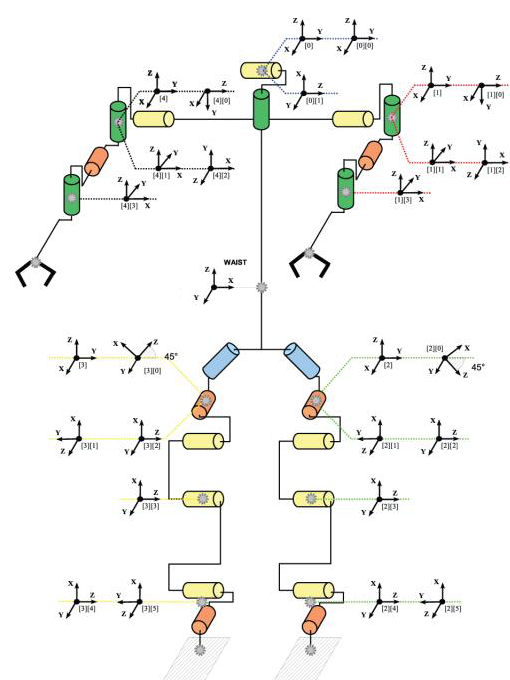
\includegraphics[scale=0.5]{figuras/nao_joints.png}
% \fonte{Retirada de \citeauthor{boedecker2008simspark}}~\label{fig:juntasNAO}
% \end{figure}

% Tabelas também devem ser referenciadas no texto e utilizadas como parte da explicação ou análise desenvolvida no capítulo. Deve ser referenciada como a Tabela~\ref{tab:tabelaTeste}. Observe que tanto figuras como tabelas devem ter suas legendas antes e a fonte indicada imediatamente após a figura ou tabela. Mesmo quando for criada pelo autor isto deve obrigatoriamente ser indicado segundo as normas da ABNT. As legendas devem ser auto-explicativas de forma que alguém que olhe a figura ou tabela e leia sua legenda consiga compreender tudo que vê sem necessidade de recorrer ao texto. O texto deve aprofundar e detalhar esta explicação, até repetindo algumas coisas que estão na legenda, mas principalmente vinculando à sequencia lógica do que está sendo exposto no texto.

% %%tabela
% \begin{table}[htb]
% \caption{Primeira tabela.}
% \begin{center}
% \begin{tabular}{|c|c|c|}
% \hline
% coluna 1 & coluna 2 & coluna 3 \\
% \hline
% valor 1,1 & valor 1,2 & valor 1,3 \\
% valor 2,1 & valor 2,2 & valor 2,3 \\
% \hline
% \end{tabular}
% \end{center}
% \fonte{Criada pelo autor.}
% \label{tab:tabelaTeste}
% \end{table}

%  Equações devem aparecer como parte natural do texto. Por exemplo energia pode ser definida como:

% %%equacao
% \begin{equation}
% E = m \times c^2,
% \label{eq1}
% \end{equation}

% \noindent onde $E$ é a energia, $m$ é a massa e $c$ é a velocidade da luz. Desta forma, apesar de numeradas, no local onde a equação aparece não será citada pelo número e sim como parte integrante do texto. Entretanto, às vezes é necessário fazer referência novamente à equação em um ponto posterior do texto (em outra seção ou mesmo em outro capítulo, ou num ponto mais distante dentro da mesma seção depois da ocorrência da mesma). Neste caso é usada a referência à Equação \eqref{eq1}.


% \section{Seção 2 do Capítulo 1 - Citações}
% Num texto científico é muito comum citar diversos autores lidos ou estudados. São feitas citações a livros, artigos científicos, etc. As normas ABNT regulamentam o formato das citações.

% São dois tipos de citações: diretas e indiretas. As citações diretas são feitas quando repete-se o texto citado igual ao original, com as mesmas palavras. Ou seja, a citação direta é uma cópia do trecho citado literalmente.

% Se a citação direta tiver menos que três linhas, deve ser feita entre aspas, assim: \foreignlanguage{english}{"This is one of the oldest leagues in RoboCupSoccer"}\cite{RoboCup}. Observe que se sua fonte for um texto em inglês ou outro idioma estrangeiro, deve se reproduzido no mesmo idioma original numa citação direta. Se você traduzir, isto vira uma citação indireta.

% Outro formato de citação direta é quando ela tem três ou mais linhas. Aí deve ser feita desta forma:
% \begin{citacao}[english]
% In the Humanoid League, autonomous robots with a human-like body plan and human-like senses play soccer against each other. Unlike humanoid robots outside the Humanoid League the task of perception and world modeling is not simplified by using non-human like range sensors. In addition to soccer competitions technical challenges take place. Dynamic walking, running, and kicking the ball while maintaining balance, visual perception of the ball, other players, and the field, self-localization, and team play are among the many research issues investigated in the Humanoid League. Several of the best autonomous humanoid robots in the world compete in the RoboCup Humanoid League\cite{RoboCup}.
% \end{citacao}


% Por fim, a forma mais comum de fazer uma citação é a indireta, quando você reproduz as ideias de um texto lido com as suas palavras. Ou seja, você não copia literalmente o texto de um autor, mas sim suas idéias, reescrevendo-as com suas palavras e de forma que faça sentido logicamente no seu texto. Isto vale inclusive para o caso em que reescrevemos em português as ideias de um texto lido em outro idioma. Neste caso a citação pode vir simplesmente logo ao final da ideia reproduzida, assim\cite{Alamdari2017}. Em alguns casos, você quer usar os autores como sujeito ou objeto de uma sentença. Por exemplo, quer dizer que \citeauthor{Xu2017} apresentaram alguma ideia ou ainda falar sobre algo que foi apresentado por \citeauthor{shafii2015learning}.


% Outra coisa comum é o uso de siglas (acrônimos). Ao utilizar uma sigla pela primeira vez, a mesma deve aparecer por extenso, assim: \gls{US}. Nas próximas ocorrências a sigla já aparecerá apenas como acrônimo, veja: \gls{US}. Qualquer nova sigla - como \gls{AA} - seguirá esta regra. Observe que siglas em inglês serão colocadas em itálico. Ao usar as siglas, as mesmas serão exibidas na Lista de siglas e abreviaturas entre os elementos pré-textuais.
